\documentclass{article}

\usepackage[margin=1in]{geometry}
\usepackage{amsmath,amsthm,tikz,fancyhdr,bm,enumitem,amssymb,empheq}
\usepackage{esint}

\theoremstyle{definition}

\newcommand*\widefbox[1]{\fbox{\hspace{2em}#1\hspace{2em}}}

\newtheorem{innercustomgeneric}{\customgenericname}
\providecommand{\customgenericname}{}
\newcommand{\newcustomtheorem}[2]{%
  \newenvironment{#1}[1]
  {%
   \renewcommand\customgenericname{#2}%
   \renewcommand\theinnercustomgeneric{##1}%
   \innercustomgeneric
  }
  {\endinnercustomgeneric}
}

\newcustomtheorem{prob}{Problem}
\newcustomtheorem{customlemma}{Lemma}

\pagestyle{fancy}
\fancyhf{}
\rhead{Lukas Zamora}
\chead{Homework 10}
\lhead{MATH 412}
\cfoot{\thepage}

\title{MATH 412 -- Homework 10}
\author{Lukas Zamora}
\date{December 3, 2018}

\setlength\parindent{0pt}


\begin{document}

    \maketitle
    
    \begin{prob}{9.2.2} $  $ \vspace{3mm} \\
        Solving
        \begin{align*}
            &c\rho\frac{\partial u}{\partial t} = \frac{\partial}{\partial x} \left( K_0 \frac{\partial u}{\partial x} \right) + Q(x,t) \\
            &u(0,t) = u(L,t) = 0 \quad u(x,0) = g(x)
        \end{align*}
        Let 
        \[
            u(x,t) = \sum\limits_{n=0}^{\infty} a_n(t) \phi_n
        \]
        Plugging into the PDE yields
        \begin{align*}
            \sum\limits_{n=0}^{\infty} \frac{da_n(t)}{dt}c\rho\phi_n &= \frac{\partial}{\partial x} \left( K_0 \frac{\partial u}{\partial x} \right) + Q(x,t) \\
            \frac{da_n(t)}{dt} &= \dfrac{\int_0^L \frac{\partial}{\partial x} \left( K_0 \frac{\partial u}{\partial x} \right) \phi_n \, dx + \int_0^L Q(x,t) \phi_n \, dx}{\int_0^L \left( \phi_n \right)^2 c\rho \, dx}
        \end{align*}
        We can use Green's formula on the first integral in the numerator:
        \begin{align*}
            \int_0^L \frac{\partial}{\partial x} \left( K_0 \frac{\partial \phi_n}{\partial x} \right) - \phi_n \frac{\partial}{\partial x}\left( K_0 \frac{\partial u}{\partial x} \right) \, dx &= u \frac{d\phi_n}{dx} - \phi_n  \left. \frac{\partial u}{\partial x} \right|_{0}^{L} \\
            -\lambda_n \int_0^L uc\rho\phi_n \, dx - \int_0^L \frac{\partial}{\partial x} \left( K_0 \frac{\partial u}{\partial x} \right) \phi_n \, dx &= 0 \\
            \int_0^L \frac{\partial}{\partial x} \left( K_0 \frac{\partial u}{\partial x} \right) \phi_n \, dx &= -\lambda_n \int_0^L uc\rho\phi_n \, dx
        \end{align*}
        We then have
        \begin{align*}
            \frac{da_n(t)}{dt} &= -\lambda_n \dfrac{ \int_0^L uc\rho\phi_n \,dx}{ \int_0^L c\rho(\phi_n)^2 \, dx} + \dfrac{ \int_0^L Q(x,t)c\rho\phi_n \, dx}{ \int_0^L c\rho(\phi_n)^2 \,dx} \\
            &= -\lambda_n a_n(t) + q_n(t)
        \end{align*}
        This is just a linear first order ODE. By using an integrating factor, we have
        \[
            a_n(t) = a_n(0)e^{-\lambda_n t} + e^{-\lambda_n t} \int_0^t q_n(\bar{t}) e^{\lambda \bar{t}} \, d\bar{t}
        \]
        where
        \[
            a_n(0) = \dfrac{ \int_0^L c\rho g(x)\phi_n \, dx}{ \int_0^L c\rho (\phi_n)^2 \, dx}
        \]
        Thus
        \[
            u(x,t) = \sum\limits_{n=0}^{\infty} \left( \dfrac{ \int_0^L c\rho g(x)\phi_n \, dx}{ \int_0^L c\rho (\phi_n)^2 \, dx} e^{-\lambda_n t} + e^{-\lambda_n t} \int_0^t \dfrac{ \int_0^L Q(x,t)c\rho\phi_n \, dx}{ \int_0^L c\rho(\phi_n)^2 \,dx} e^{\lambda_n \bar{t}} \, d\bar{t} \right)\phi_n
        \]
        By changing the order of summation and integrating, we have
        \[
            u(x,t) = \int_0^L g(\bar{x}) \sum\limits_{n=0}^{\infty} \left( \frac{\phi_n(\bar{x})\phi_n(x) e^{-\lambda_n t} c\rho}{\int_0^L c\rho (\phi_n)^2 \, dx} \right) \, d\bar{x} + \int_0^t \int_0^L Q(\bar{x},\bar{t}) \sum\limits_{n=1}^{\infty}\left( \frac{\phi_n(\bar{x})\phi_n(x) e^{-\lambda_n (t-\bar{t})} c\rho}{\int_0^L c\rho (\phi_n)^2 \, dx} \right) \, d\bar{x} \, d\bar{t}
        \]
        If we let our Green function to be
        \[
            G(x,t;\bar{x},\bar{t}) = \sum\limits_{n=1}^{\infty}\left( \frac{\phi_n(\bar{x})\phi_n(x) e^{-\lambda_n (t-\bar{t})} c\rho}{\int_0^L c\rho (\phi_n)^2 \, dx} \right)
        \]
        we obtain
        \[
            \boxed{ u(x,t) = \int_0^L g(\bar{x}) G(x,t;\bar{x},0) \, d\bar{x} + \int_0^t \int_0^L Q(\bar{x},\bar{t})G(x,t;\bar{x},\bar{t}) \, d\bar{x} \, d\bar{t} }
        \]
        $ $
    \end{prob}
    
    \begin{prob}{9.3.5} $ $ \vspace{2mm} \\
        $ \dfrac{d^2 u}{dx^2} = f(x) \quad u(0) = \dfrac{du}{dt}(L)=0 $ \\
        \begin{enumerate}[label=\alph*.)]
            \item Integrating twice, we have
                \begin{align*}
                    u(x) - u(0) &= \int_0^x \int_L^{x_0} f(\bar{x}) \, d\bar{x} \, dx_0 \\
                    u(x) &= \int_0^x \int_L^{x_0} f(\bar{x}) \, d\bar{x} \, dx_0
                \end{align*}
                Integrating by parts,
                \begin{align*}
                    u(x) &= x_0 \left. \int_L^{x} f(\bar{x}) \, d\bar{x} \right|_L^x - \int_0^x x_0 f(x_0) \, dx_0 \\
                    &= \boxed{ x\int_L^{x} f(\bar{x}) \, d\bar{x} - \int_0^x x_0 f(x_0) \, dx_0 }
                \end{align*}

            \item Consider a basis of homogeneous solutions $u_{1} = x, u_{2} = 1$. The general solution is then
            \begin{align*}
                u &= u_1 v_1 + u_2 v_2 \\
                  &= x\int_0^x f(x_0) \, dx_0 - \int_0^x x_0 f(x_0) \, dx_0 + c_1x + c_2 \\
                u(0) &= 0 = c_2 \\
                \frac{du}{dx}(L) &= 0 = \int_0^L f(x_0) \, dx_0 + L(f(x_0)) \Big|_0^L - \int_0^L x_0 f(x_0) \, dx_0 + c_1 \\
                &\Rightarrow c_1 = -\int_0^L f(x_0) \, dx_0
            \end{align*}
            Thus
            \begin{align*}
                u(x) &= x\int_0^x f(x_0) \, dx_0 - \int_0^x x_0 f(x_0) \, dx_0 - x\int_0^L f(x_0) \, dx_0 \\
                &= \boxed{ \int_0^x (x-x_0) f(x_0) \, dx_0 - x\int_0^L x_0 f(x_0) \, dx_0 }
            \end{align*}

            \item
                \[
                    u(x) = -\int_x^L x f(x_0) \, dx_0 - \int_0^L x_0 f(x_0) \, dx_0
                \]
                \begin{empheq}[box=\fbox]{align*}
                    u(x) &= \int_0^L f(x_0) G(x,x_0) \, dx_0 \\
                    G(x,x_0) &= \begin{cases} -x &x<x_0 \\ -x_0 & x_0 > x  \end{cases}
                \end{empheq}

            \item Our eigenfunction is 
                \[
                    \phi_n = \sin(\sqrt{\lambda_n} x) \, , \quad \lambda_n = \left( \frac{(2n+1)\pi}{2L} \right)^2
                \]
                Let 
                \[
                    u(x) = \sum\limits_{n=0}^{\infty} a_n \sin(\lambda_n x)
                \]
                and plug into the ODE to obtain
                \[
                    -\sum\limits_{n=0}^{\infty} a_n \lambda_n \sin(\sqrt{\lambda_n} x) = f(x)
                \]
                By orthogonality, we have
                \[
                    a_n = -\frac{\int_0^L f(x) \sin(\sqrt{\lambda_n} x) \, dx}{\lambda_n \int_0^L \left(  \sin(\sqrt{\lambda_n} x) \right)^2 \, dx}
                \]
                Thus
                \[
                    u(x) = \sum\limits_{n=0}^{\infty} - \frac{\int_0^L f(x_0) \sin(\sqrt{\lambda_n} x_0) \sin(\lambda_n x) \, dx_0}{\lambda_n \int_0^L \left( \sin(\sqrt{\lambda_n} x) \right)^2 \, dx}
                \]
                By changing the order of summation and integrating, we have
                \[
                    u(x) = \int_0^L f(x_0) \sum\limits_{n=0}^{\infty} \frac{\sin(\sqrt{\lambda_n} x_0) \sin(\lambda_n x) \, dx_0}{-\lambda_n \int_0^L \left( \sin(\sqrt{\lambda_n} x) \right)^2 \, dx}
                \]
                Thus
                \begin{empheq}[box=\fbox]{align*}
                    u(x) &= \int_0^L f(x_0) G(x,x_0) \, dx_0 \\
                    G(x,x_0) &= \sum\limits_{n=0}^{\infty} \frac{\sin(\sqrt{\lambda_n} x_0) \sin(\lambda_n x)}{-\lambda_n \int_0^L \left( \sin(\sqrt{\lambda_n} x) \right)^2 \, dx}
                \end{empheq}
        \end{enumerate}
        $ $
    \end{prob}
    

    \begin{prob}{9.3.6} $ $ \vspace{2mm} \\
        $ \dfrac{d^2 G}{dx^2} = \delta(x-x_0) \quad G(0,x_0) = \dfrac{dG}{dx}(L,x_0)=0 $ \\
        \begin{enumerate}[label=\alph*.)]
            \item If $x\neq x_{0}$, we have
                \[
                    \frac{d^2G}{dx^2} = 0
                \]
                Thus the solution is the following
                \[
                    G(x,x_0) = \begin{cases} c_1x + c_2 &x<x_0 \\ d_1x + d_2 & x>x_0 \end{cases}
                \]
                Applying boundary conditions,
                \begin{align*}
                    G(0,x_0) &= 0 = c_2 \\
                    \frac{dG}{dx}(L,x_0) &= 0 = d_1
                \end{align*}
                If $G$ is continuous at $x=x_{0}$, $c_1x_{0}=d_{2}$. Integrating the ODE, we have
                \begin{align*}
                    \left. \frac{dG}{dx} \right|_{x_0^-}^{x_0^+} &= \int_{x_0^-}^{x_0^+} \delta(x-x_0) \, dx \\
                    \frac{dG}{dx}(x_0^+) - \frac{dG}{dx}(x_0^-) = 1 \\
                    0 - c_1 &= 1 \\
                    c_1 &= -1, \; d_2 = -x_0
                \end{align*}
                Thus
                \[
                    \boxed{ G(x,x_0) = \begin{cases} -x & x<x_0 \\ -x_0 & x>x_0  \end{cases} }
                \]
            \item The graph of $G(x,x_{0}) = G(x_{0},x)$
                \begin{center}
                    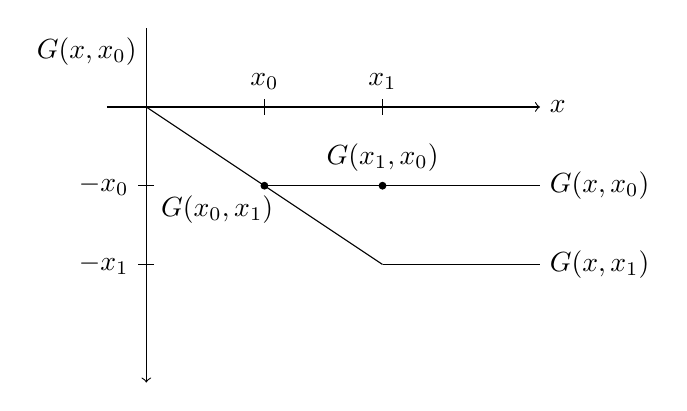
\begin{tikzpicture}
                        \draw[<-] (-1,-4.5) -- (-1,0) node[below left] {$G(x,x_{0})$};
                        \draw[->] (-1.5,-1) -- (4,-1) node[right] {$x$};
                        \draw (0.5,-0.9) -- (0.5,-1.1) node[above=2mm] {$x_{0}$};
                        \draw (2,-0.9) -- (2,-1.1) node[above=2mm] {$x_{1}$};
                        \draw (-0.9,-2) -- (-1.1,-2) node[left] {$-x_{0}$};
                        \draw (-0.9,-3) -- (-1.1,-3) node[left] {$-x_{1}$};
                        \node[circle,fill,inner sep=1pt] at (0.5,-2) {};
                        \node at (-0.1,-2.3) {$G(x_0,x_1)$};
                        \node[circle,fill,inner sep=1pt,label=above:{$G(x_1,x_0)$}] at (2,-2) {};
                        \draw (0.5,-2) -- (4,-2) node[right] {$G(x,x_0)$};
                        \draw (-1,-1) -- (2,-3);
                        \draw (2,-3) -- (4,-3) node[right] {$G(x,x_1)$};
                    \end{tikzpicture}
                \end{center}
            \item The Green function is the same as $G(x,x_{0})$ solved for in part (a).
        \end{enumerate}
        $ $
    \end{prob}

    \begin{prob}{9.3.11} $ $ \vspace{2mm} \\
        $ \dfrac{d^2 G}{dx^2} + G = \delta(x-x_0) \quad G(0,x_0) = G(L,x_0)=0 $ \\
        \begin{enumerate}[label=\alph*.)]
            \item If $x\neq x_{0}$, then we have
                \[
                    \frac{d^2G}{dx^2} + G = 0
                \]
                which has the following general solution
                \[
                    G(x,x_0) = \begin{cases} A\cos(x) + B\sin(x) &x<x_0 \\ C\cos(x) + D\sin(x) & x>x_0 \end{cases}
                \]
                Applying boundary conditions,
                \begin{align*}
                    G(0,x_0) &= 0 = A \\
                    G(L,x_0) &= 0 = C\cos(L) + D\sin(L) \\
                    C &= -D\tan(L)
                \end{align*}
                If $G$ is continuous at $x=x_{0}$, we have
                \begin{align*}
                    B\sin(x_0) &= -D\tan(L)\cos(x_0) + D\sin(x_0) \\
                             B &= -D\tan(L)\cot(x_0) + D \\
                             B &= D(1-\tan(L)\cot(x_0))
                \end{align*}
                Integrating the ODE, we have
                \begin{align*}
                    \left. \frac{dG}{dx} \right|_{x_0^-}^{x_0^+} + \int_{x_0^-}^{x_0^+} G \, dx &= \int_{x_0^-}^{x_0^+} \delta(x-x_0) \, dx \\
                    \frac{dG}{dx}(x_0^+) - \frac{dG}{dx}(x_0^-) &= 1 \\
                    D\tan(L)\sin(x_0) + D\cos(x_0) - D(1-\tan(L)\cot(x_0))\cos(x_0) &= 1 \\
                    D\tan(L) &= \sin(x_0) \\
                    D &= \frac{\sin(x_0)}{\tan(L)}
                \end{align*}
                Thus 
                \[
                    \boxed{ G(x,x_0) = \begin{cases} \dfrac{\sin(x_0)}{\tan(L)}(1-\tan(L)\cot(x_0))\sin(x) & x<x_0 \\ -\sin(x_0)\cos(x) + \dfrac{\sin(x_0)}{\tan(L)}\sin(x) &x>x_0 \end{cases} }
                \]
                We needed to assume $L\neq n\pi$ because $\tan(x) = 0$ for $x=n\pi, n \in \mathbb{Z}$.
            \item From $G(x,x_{0})$, 
                \[
                    G(x_0,x) = \begin{cases} \dfrac{\sin(x)}{\tan(L)}(1-\tan(L)\cot(x))\sin(x_0) &x>x_0 \\ -\sin(x)\cos(x_0) + \dfrac{\sin(x)}{\tan(L)}\sin(x_0) & x<x_0 \end{cases}
                \]
                For $x>x_{0}$ we need the following to be true
                \begin{align*}
                    -\sin(x_0)\cos(x) + \frac{\sin(x_0)}{\tan(L)}\sin(x) &= \frac{\sin(x)}{\tan(L)}(1-\tan(L)\cot(x))\sin(x_0) \\
                    &= \left( \frac{\sin(x)}{\tan(L)} - \sin(x) \frac{\cos(x)}{\sin(x)} \right) \sin(x_0) \\
                    &= \frac{\sin(x)}{\tan(L)}\sin(x_0) - \cos(x)\sin(x_0)
                \end{align*}
                For $x<x_{0}$ we need the following to be true
                \begin{align*}
                    -\sin(x)\cos(x_0) + \frac{\sin(x)}{\tan(L)}\sin(x_0) &= \frac{\sin(x_0)}{\tan(L)}(1-\tan(L)\cot(x_0))\sin(x) \\
                    &= \left( \frac{\sin(x_0)}{\tan(L)} - \sin(x_0) \frac{\cos(x_0)}{\sin(x_0)} \right) \sin(x) \\
                    &= \frac{\sin(x_0)}{\tan(L)}\sin(x) - \cos(x_0)\sin(x)
                \end{align*}
                Thus $G(x,x_{0}) = G(x_{0},x)$.
        \end{enumerate}
        $ $
    \end{prob}

    \newpage

    \begin{prob}{9.3.21} $ $ \vspace{2mm} \\
        Solving
        \[
            \frac{dG}{dx} = \delta(x-x_0) \quad G(0,x_0)=0
        \]
        By integrating the ODE, we have
        \begin{align*}
            G(x,x_0) \bigg|_{x_0^-}^{x_0^+} &= \int_{x_0^-}^{x_0^+} \delta(x-x_0) \, dx \\
            &= 1
        \end{align*}
        Since there is a jump at $x=x_{0}$ we have
        \[
            \boxed{ G(x,x_0) = \begin{cases} 0 &x<x_0 \\ 1 &x>x_0 \end{cases} }
        \]
        The result of the delta function $\delta(x-x_{0})$ is symmetric, i.e. $\delta(x-x_{0}) = \delta(x_{0}-x)$. Taking the boundary condition $G(x_{0},0) = 0$ for $G(x_{0},x)$ and doing the same steps as above results in $G(x,x_{0}) \neq G(x_{0},0)$. So $G(x,x_{0})$ is not symmetric.
    \end{prob}

\end{document}